%\setlength{\epigraphwidth}{0.5\textwidth}
%\epigraph{There is an art in the contemplation of water. It is necessary to look at it as foaming in waves.}{--- \textup{Mencius}, \textit{\\translated by James Legge}}

The SNO+ water phase data were taken from May 2017 to September 2018. The period from May 2017 to October 2018 is the first stage of the water phase. During this stage, several calibration runs were taken, including the $^{16}$N calibration scans and the laserball scans. During the period from October 2018 to July 2019, over 20 tonnes of LAB (without PPO) was filled into the detector and the LAB mostly occupied the neck volume, slightly below the neck bottom. With the nitrogen cover gas on the top of the AV, the dataset taken during this period is called ``low background dataset''. In this study, 4838 runs of data were used, which summed up a total live time of 190.31 days after the data cleaning process.
 
In this chapter, I applied the MPW reconstruction algorithm mentioned in Chapter 4 as a position and direction fitter to the raw dataset as well as the run-by-run MC simulations. The fitted event vertex was used by the energy fitter developed by the SNO+ collaboration.  

I mainly analyzed the low background dataset. 

extract the $^8$B solar neutrino flux and interaction rate


to search for these events
then convert into the interaction rate as well as the $^8$B solar neutrino flux.




Monte Carlo simulations were produced by the RAT software, which was described in \ref{sect:rat}.

compare to SuperK results.


data cleaning and analysis cuts 

The analysis cuts depend on the reconstructed results.


\section{Detector Backgrounds}

\subsection{Physics Backgrounds}

Radioactive Isotopes

assays


in-situ
ex-situ

the instrumental backgrounds can be removed by the data-cleaning approaches.



\subsection{Instrumental Backgrounds}





\section{High Level Cuts: Classifiers}

A set of classifiers were developed by SNO analysis and been optimized for the SNO+ water analysis\cite{highlevel}.

valid reconstruction


These classifiers utilize the reconstructed quantities

\begin{itemize}

\item[$\bullet$] In time ratio (ITR) classifier

For each event, this classifier loops the triggered PMTs (hits), calculates the $t_{res}$ and then finds the ratio of the number of hits in an optimized prompt time window. In the water phase, it checked 

[-2.5,5.0]~ns (for the water phase) to the total number of hits.


\item[$\bullet$] $\beta_{14}$ isotropy classifier

This classifier uses Legendre polynomials to return the	first ($\beta_1$) and the fourth ($\beta_4$) spherical	harmonics of an event, where:
\[
\beta_l = \frac{2}{N(N-1)}\sum_{i=1}^{N-1}\sum_{j=i+1}^N P_l(\cos\theta_{ij})
\]
and $P_l(\cos\theta_{ij})$ are Legendre polynomials.


The	combination	of these two polynomials returned by the classifier	was	
practically	chosen by the SNO collaboration	to be: $\beta_{14}=\beta_1+4\beta_4$
as this gives gaussian-like	distribution pattern for Cherenkov events.	
Essentially	any	deviation from zero suggests some polarity (i.e. the event is not isotropic).	


\item[$\bullet$] $\theta_{ij}$ isotropy classifier 

describes the angle subtended at an event vertex by PMT \#i and PMT \#j.

\[
\cos\theta_{ij}=\frac{(\vec{X}_{PMT\#i}- \vec{X}_{event})\cdot (\vec{X}_{PMT\#j}- \vec{X}_{event})}{|\vec{X}_{PMT\#i}- \vec{X}_{event}||\vec{X}_{PMT\#j}- \vec{X}_{event}|}
\]


\item[$\bullet$] Kullback–Leibler (KL) divergence for Cherenkov distribution. The KL divergence is also called ``relative entropy'' and it is used to measure the dissimilarity of two probability distributions\cite{murphy2012machine}. I used this quantity to compare the reconstructed angular distribution of a random event with the assumed Cherenkov distribution of solar $\nu_e$ events extracted from simulation to check the dissimilarity of the event compared to the solar $\nu_e$ event. The quantity $D_{KL}(p||q)$ is calculated as: 
\begin{equation}\label{kldiv}
KLdiv(p||q) \equiv \sum_{i}^N p(x_i)\log{\frac{p(x_i)}{q(x_i)}},
\end{equation}

where $p(x_i)$ is the histogramme distribution of $(\vec{X}_{PMT}-\vec{X}_{fit})/|\vec{X}_{PMT}-\vec{X}_{fit}|\cdot\vec{u}_{fit}$ 



with a time residual window cut $[-5,1]~ns$.







\end{itemize}





The output values were used for distinguishing the signal from backgrounds.


\section{Solar \texorpdfstring{$\nu_e$}{Lg} Analysis and Background Separation in Water Phase}

solar neutrino candidate events in the open dataset.

\begin{figure}[htbp]
	\centering
	\subfigure[Run 100093, GTID 11108354]{ 
		\begin{minipage}[t]{0.4\textwidth}
			\centering
			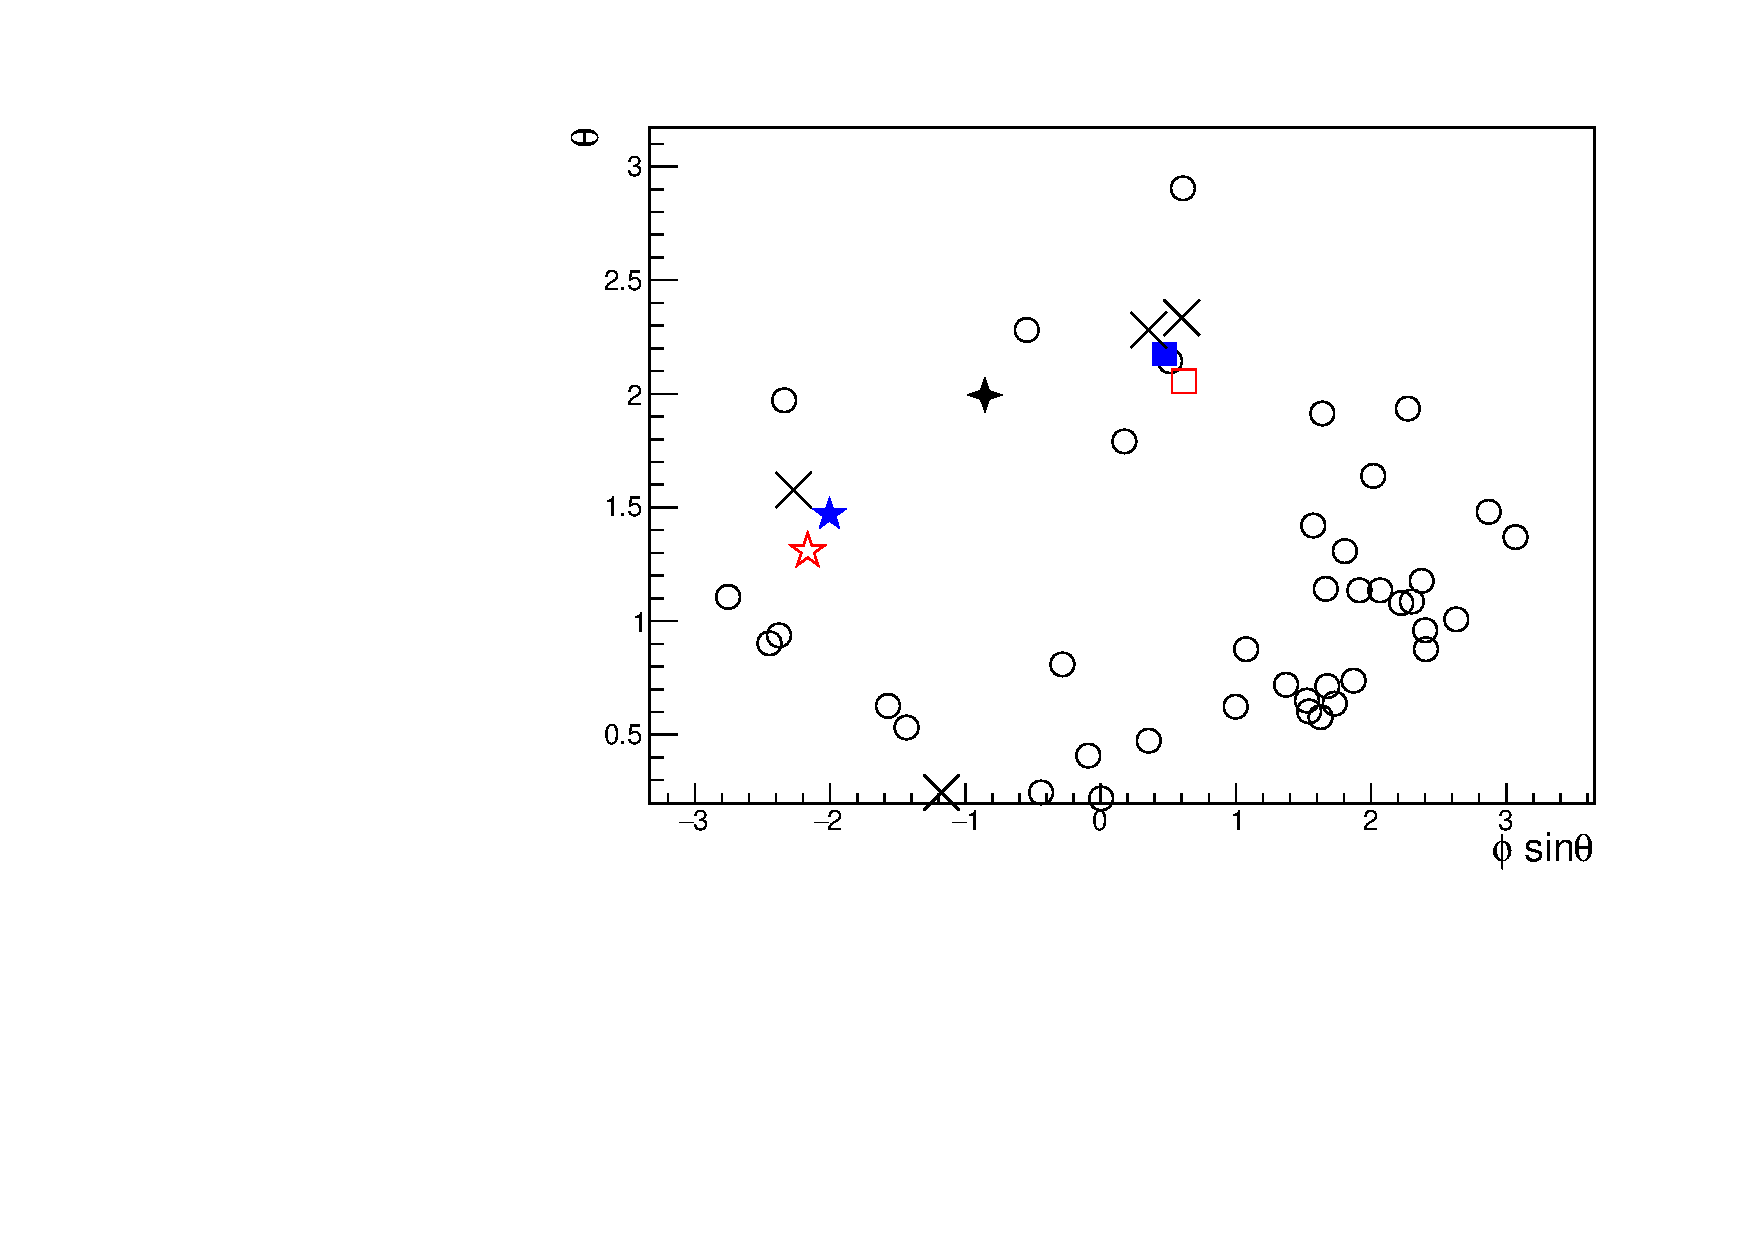
\includegraphics[width=6cm]{PMTmap_100093.pdf}
		\end{minipage}
	}
	\subfigure[Run 100207, GTID 5079885]{ 
		\begin{minipage}[b]{0.4\textwidth}
			\centering
			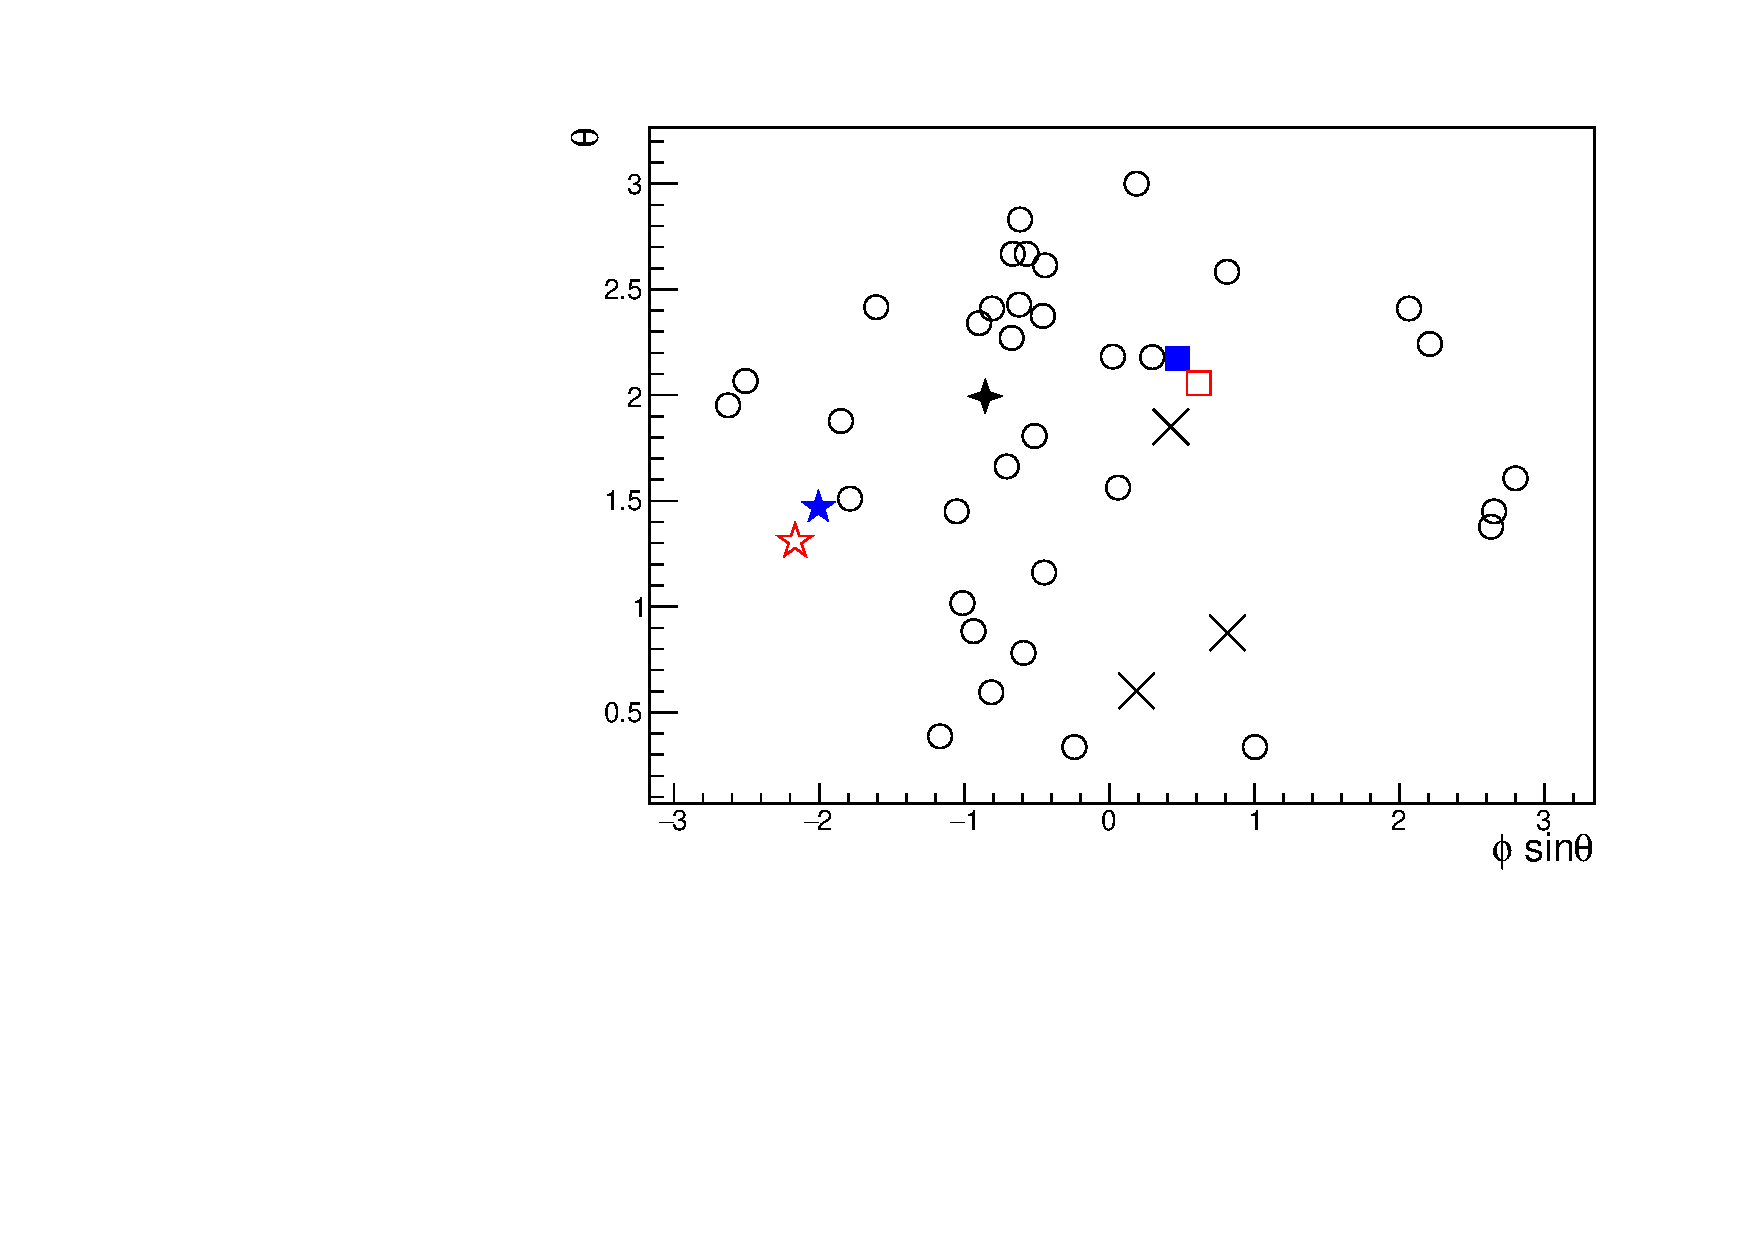
\includegraphics[width=6cm]{PMTmap_100207.pdf}
		\end{minipage}
	}
	\subfigure[Run 100632, GTID 7882360]{ 
		\begin{minipage}[t]{0.4\textwidth}
			\centering
			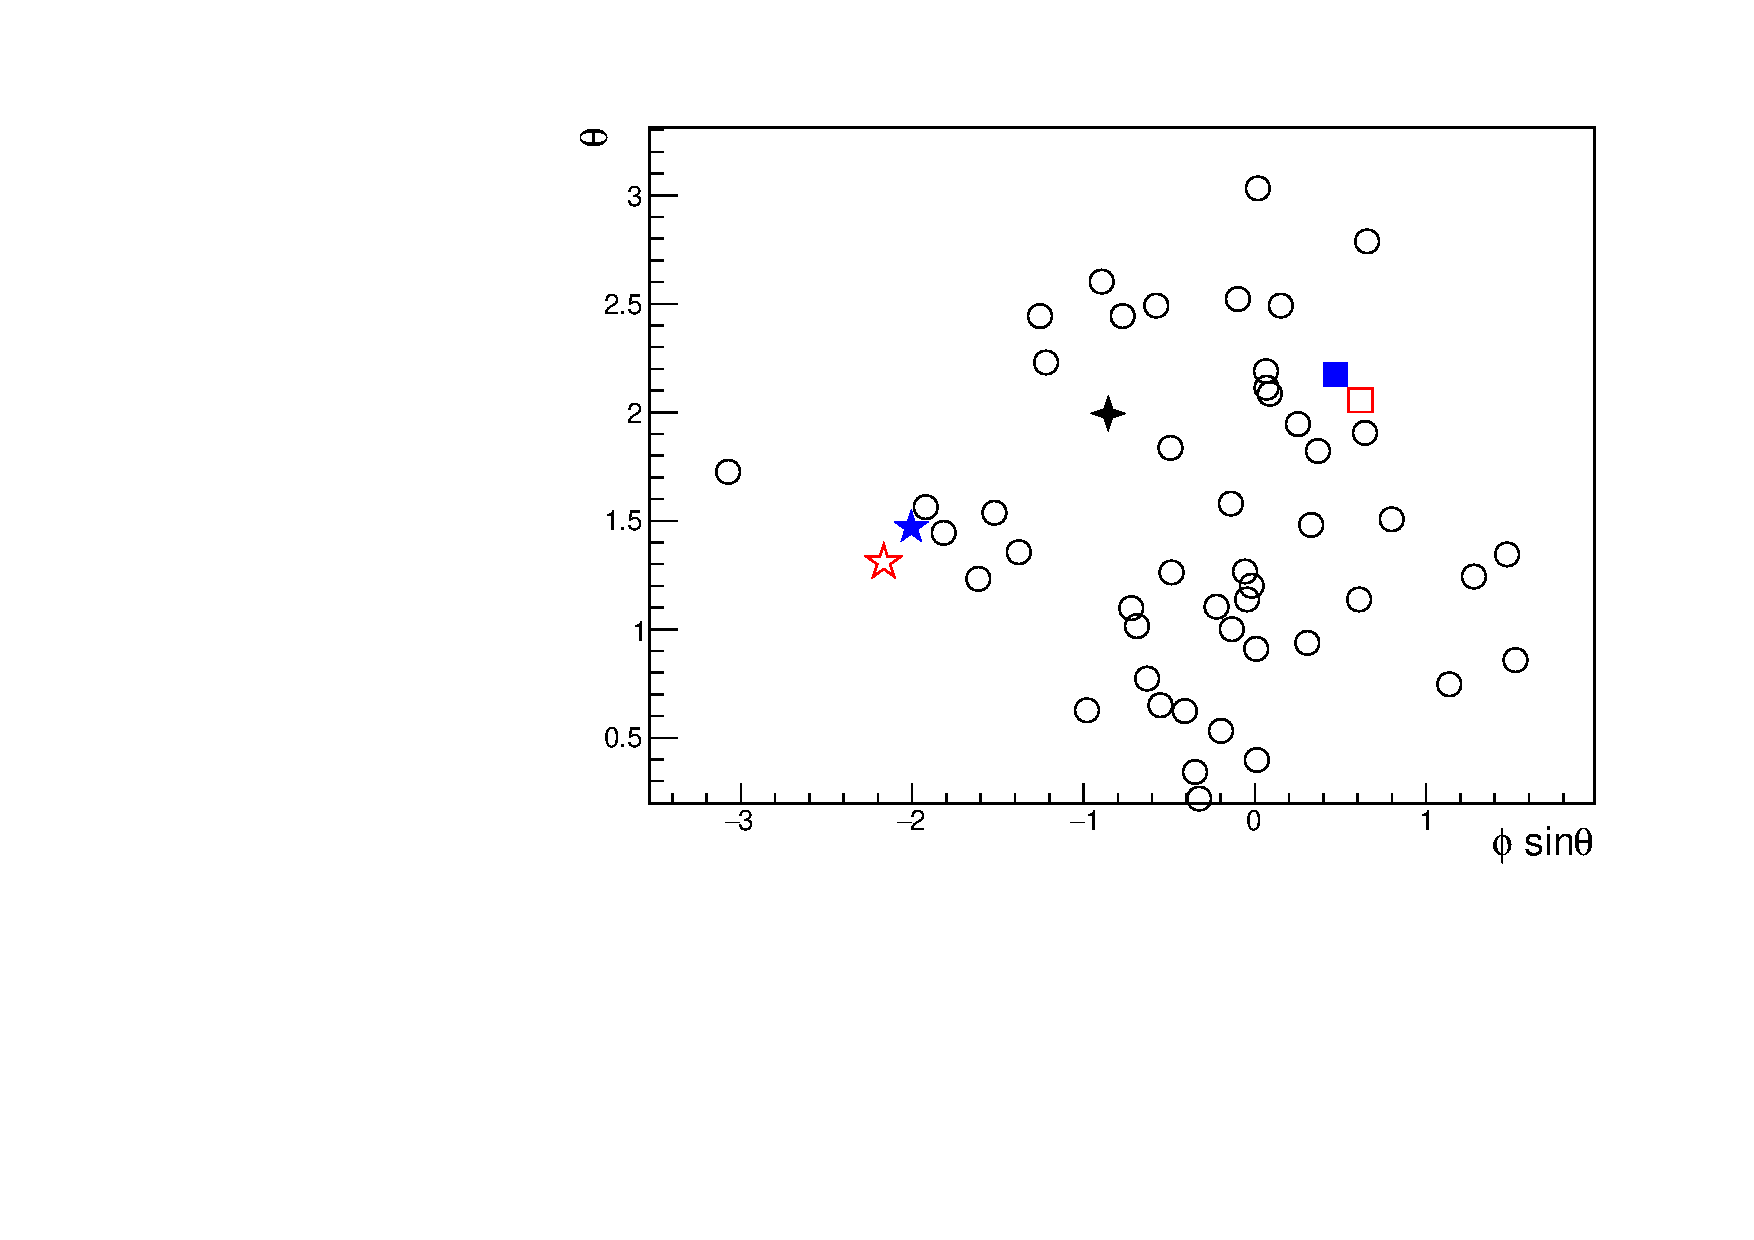
\includegraphics[width=6cm]{PMTmap_100632.pdf}
		\end{minipage}
	}
	\subfigure[Run 100663, GTID 15767175]{ 
		\begin{minipage}[t]{0.4\textwidth}
			\centering
			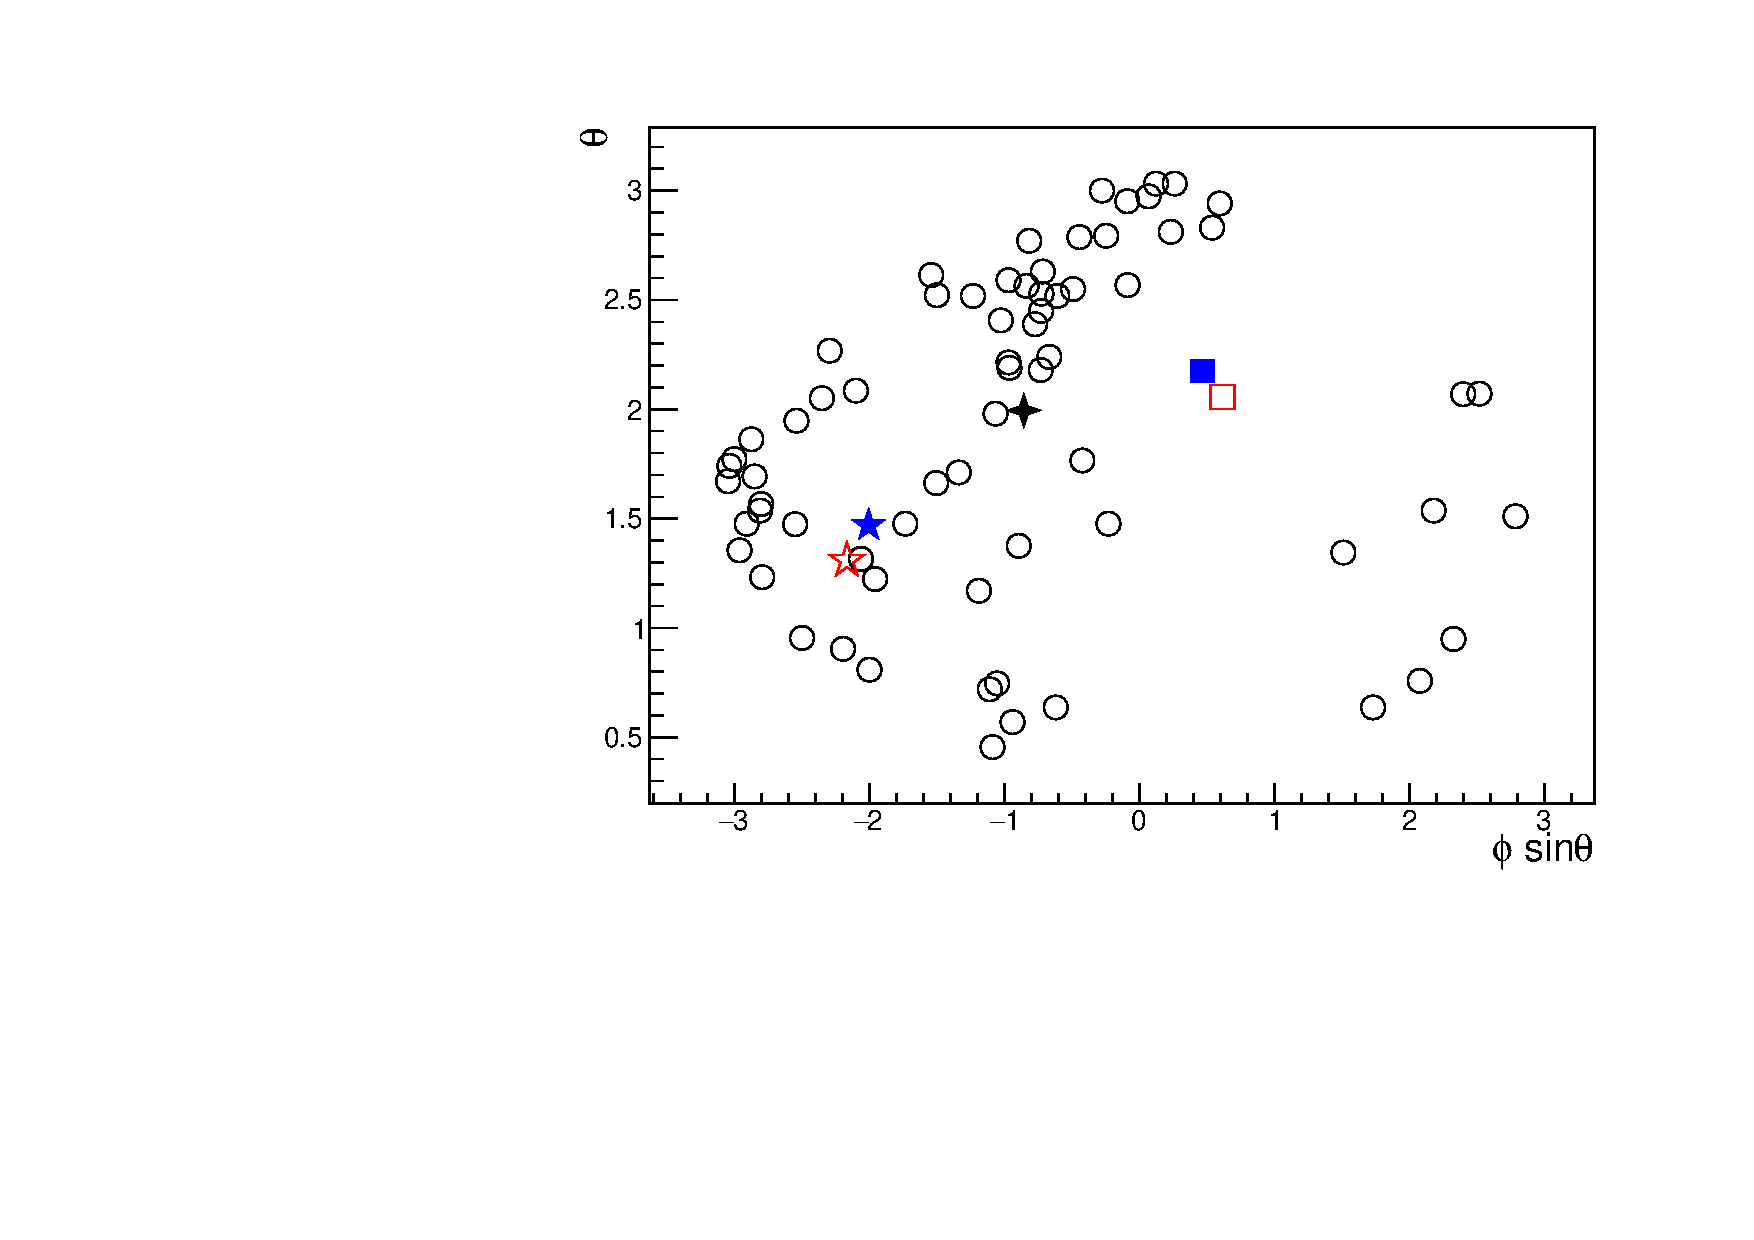
\includegraphics[width=6cm]{PMTmap_100663.pdf}
		\end{minipage}
	}
	\subfigure[Run 100915, GTID 169700]{ 
		\begin{minipage}[t]{0.4\textwidth}
			\centering
			{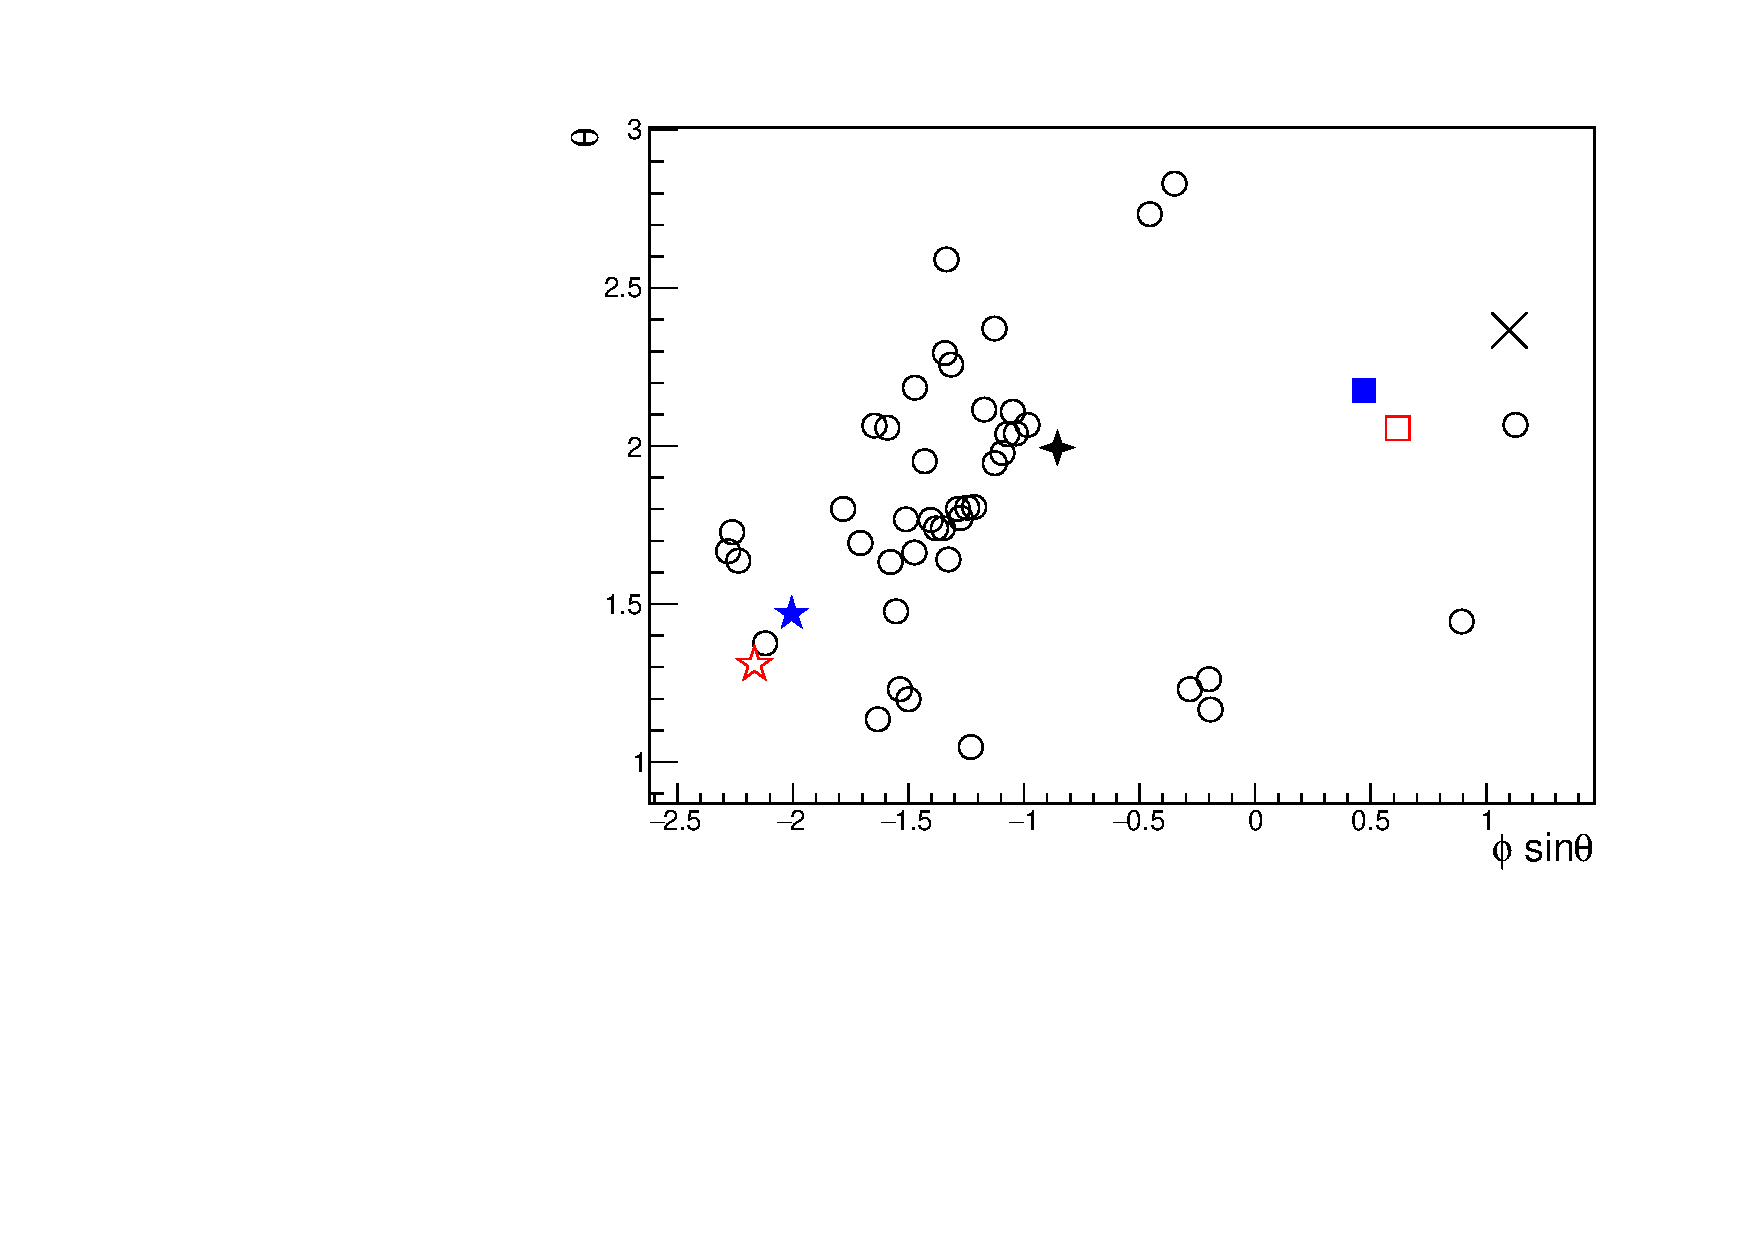
\includegraphics[width=6cm]{PMTmap_100915.pdf}}
		\end{minipage}
	}
	\subfigure[Legends]{ 
		\begin{minipage}[b]{0.4\textwidth}
			\centering
			{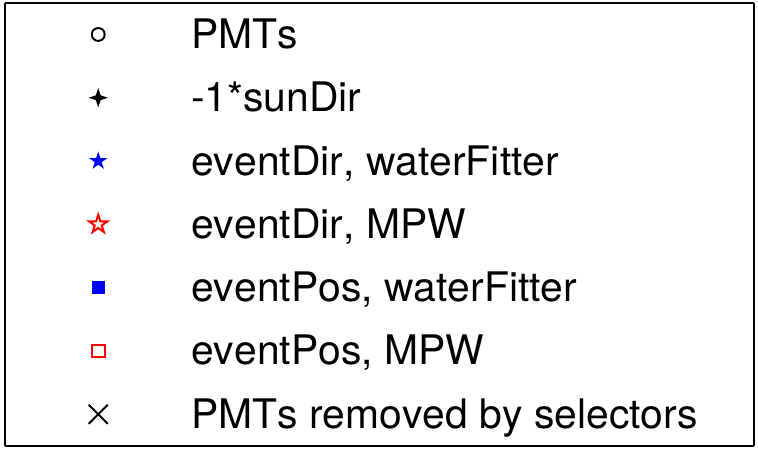
\includegraphics[width=5cm]{solarLegends.png}}
		\end{minipage}
	}
	\caption{Fit results for the candidate events, projected onto PMT sinusoidal maps. Black circles stand for
		the hit PMTs used by the fitter; crosses stand for the hit PMTs removed by the selectors; blue full star stands for the event direction fitted by the waterFitter; red open star stands for the direction fitted by the MPW; full double diamond stands for the solar direction*-1; blue full square stands for the event position fitted by the waterFitter; open square stands for the position fitted by the MPW.}
	\label{openDataSetCandidate}
\end{figure}


\subsubsection{Open Dataset Analysis}

MPW fit results

fiducial volume cut effects

\begin{table}[ht]
	\centering
	\caption{Candidate events in the open dataset. Compared the fitted results of the candidate events with different fitters.}
	\label{opendata}
	\begin{tabular*}{150mm}{c@{\extracolsep{\fill}}cccccccc}
		\toprule
	 Fitter &	Run &  GTID &  $z-0.108$(m) & $R$(m)& $(R/R_{av})^3$ & $\cos\theta_{sun}$ & SNO+ Day\\
		\hline 
	Rat & 100093 &11108354 &3.49 &3.57 &0.21 &-0.954459 &2683.92 \\	
	MPW &  --& --& 3.43 &	3.52 &	0.20	& -0.906388 & --\\
	Rat &	100207 &5079885 &-2.61 &4.60 &0.45 &0.816215 &2687.04\\
	MPW &	 --& --& -3.63 & \textbf{7.61} &	2.03 & \textbf{0.656374} & -- \\
	Rat &100632 &7882360 &1.77 &3.19 &0.15 &0.937212 &2696.93\\
	 MPW &    --& --&  1.67 & 3.11 &	0.14 & 0.910527 & -- \\
	Rat &100663 &15767175 &-4.33& 4.96 &0.56 &0.977517 &2698.18\\
	MPW & --& -- &-4.45 &	5.07 &	0.60 &	0.979943 & -- \\
	Rat &100915 &169700 &-1.00 &5.10 &0.61 &0.341287 &2701.23\\
	MPW &	--& --& -1.08 &	5.08 &	0.61 &	0.336706 & -- \\	
		\bottomrule
	\end{tabular*}
\end{table}

\begin{table}[ht]
	\centering
	\caption{Candidate events in the open dataset, searched by the MPW fitter.}
	\label{opendataMPW}
	\begin{tabular*}{150mm}{c@{\extracolsep{\fill}}cccccccc}
		\toprule
		Run & GTID & energy & $z-0.108$ & $R$ & $(R/R_{av})^3$ & $\cos\theta_{sun}$\\
		\hline 
100093 &	11108354	&5.827 & 3.43 & 3.52 & 0.20 & -0.907005\\
100632&	7882360    &6.183& 1.67 &3.11 &0.14 &0.9146124\\
100663&	15767175   &	6.182 & -4.45 &5.07 &0.60&	0.9807349\\
100915&	169700   &	5.684 &	-1.07 &5.08 &0.61&0.3385341\\
100984&	8621621&	5.701 & 0.76 &4.75 &0.502&-0.647735\\
101075&	11673714&	5.667 &4.43 &5.18 &0.64& 0.5873025\\

		\bottomrule
\end{tabular*}
\end{table}

In SNO+ water phase, solar $\nu_e$s are basically measured via elastic scattering $\nu_e+e^-\to \nu_e+e^-$. The maximum kinetic energy of the recoil electron is
$T_{max}=\frac{2E^2_\nu}{2E_\nu+m_e c^2}$
the cross section is $\sigma(\nu_e+e^-\to \nu_e+e^-)=9.52\times 10^{-44}(E_\nu/10~MeV)~cm^2$
the expected solar neutrino rate is 
$R=A\int_{T_{thresh}}^{T_{max}}\frac{d\sigma}{dE}\frac{dN}{dE_\nu}dE_\nu$.

A ``solar angle'', $\theta_{sun}$ is the direction of the event relative to the Sun's location,
$\cos\theta_{sun}\equiv \vec u_{event}\cdot (\vec{X}_{event}-\vec{X}_{sun})$, where $\vec{X}_{event}-\vec{X}_{sun}$ can be replaced by the Sun's location relative to the SNOLAB location since the whole lab can be treated as a point regarding the long distance to the Sun.


\subsection{TMVA Analysis}
The MC simulations of the realistic runs (200004 to 203602) were used. This is a sub-dataset to the whole ``low background dataset'', with a live time of 92.54 days. for testing and training the TMVA methods.

Two types of background isotopes, $^{208}$Tl and $^{214}$Bi were simulated in different detector regions. In this study, the background events simulated in the inner AV (internal backgrounds) , in the AV and in the external water region were checked. The solar $\nu_e$ events simulated in the inner AV were used as signals. Table.~\ref{table:mixed_MC} summarizes the types of simulations used in this study. 
\begin{table}[ht]
	\centering
	\caption{Datasets of MC simulations.}
	\label{table:mixed_MC}
	\begin{tabular*}{100mm}{c@{\extracolsep{\fill}}cccccccc}
		\toprule
		Simulations & Simulated positions in the detector\\
		\hline 
		$^{208}$Tl & inner AV (internal $^{208}$Tl)\\
		-- & AV \\
		-- & external water (external $^{208}$Tl)\\
		\midrule
		$^{214}$Bi & inner AV (internal $^{214}$Bi)\\
		-- & AV \\
		-- & external water (external $^{214}$Bi)\\
		\midrule
		Solar $\nu_e$ & inner AV (internal $\nu_e$)\\
		-- & AV \\
		-- & external water (external $\nu_e$)\\
		\bottomrule
	\end{tabular*}
\end{table}

Different types of the simulations were merged into a mixed dataset. The simulated solar $\nu_e$ events are tagged as signals and mixed with $^{214}$Bi and $^{208}$Tl background events. The total dataset was divided into training and testing sets. 

Fig.~\ref{TMVA_bkgs_1} shows the energy spectrum of simulated internal events with their fitted positions inside the 5.5-m fiducial volume, i.e., with a cut of $R'_{fit}<5.5~m$, where $R'_{fit}$ is the magnitude of the reconstructed event position $\vec{X}_{fit}$ in the AV coordinate, $R'_{fit}=\sqrt{x^2_{fit}+y^2_{fit}+(z_{fit}-108)^2}$. The 108 mm offset in $z$ was discussed in Chapter 3 and Chapter 4. 

\begin{figure}[!htb]
	\centering
	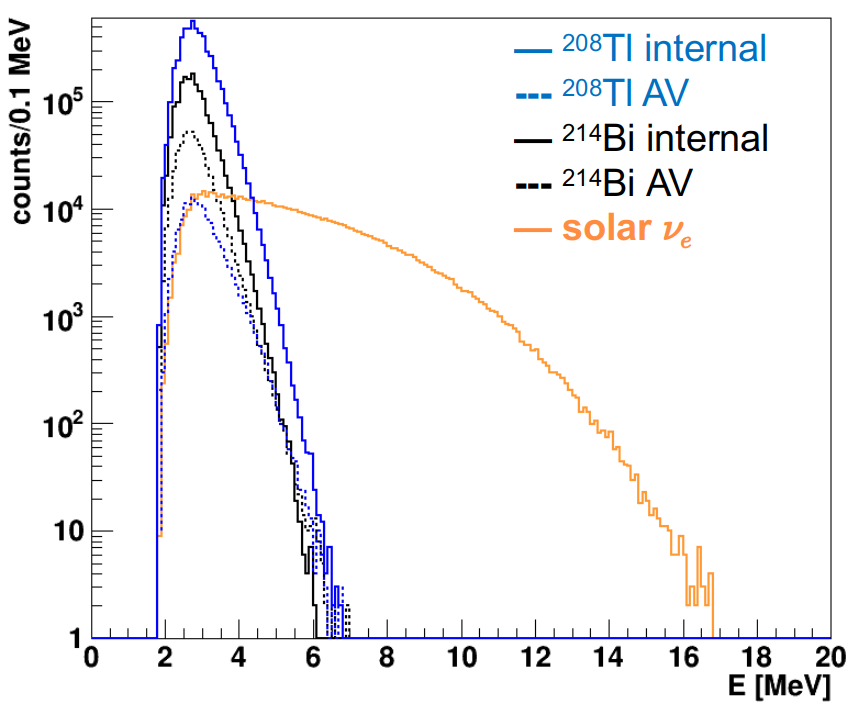
\includegraphics[width=8cm]{TMVA_bkgs_1.png}
	\caption{Energy spectrum of the simulated events for $^{214}$Bi (black), $^{208}$Tl (blue) and solar $\nu_e$ (orange). Solid lines show the internal events and dotted lines show the AV events.}
	\label{TMVA_bkgs_1}
\end{figure}

The Toolkit for Multivariate Data Analysis with ROOT (TMVA) \cite{tmvaWebsite,albertsson2007tmva}

Cuts were applied: $NHits>20$, $4<E_{fit}<15~MeV$, $R_{fit}<5500~mm$, $ITR>0.55$, $-0.12<\beta_{14}<0.95$.



In this sub-dataset, runs from 201700 to 202516 were taken as training set (69.5\% of the total sub-dataset), and the rest 30.5\% were taken as testing set. Once the weights of the parameters were tuned, they were put into the actual data.

The Fisher discriminator (Fisher), the Likelihood, the Boosted Decision Tree (BDT), and the Artificial Neural Networks Multilayer Perceptron (ANN-MLP, or MLP in short) methods implemented in the TMVA package were used\cite{albertsson2007tmva}.


The MLP method gave the best results, while it was the most CPU consuming one (about two times of the Fisher method).

9 parameters were used as inputs: $ITR$, $\beta_{14}$, $NHits$, $E_{fit}$, $DL_{}$ and $\hat u \cdot \hat R$.



 for the multiple variable analysis (MVA).

A Receiver Operating Characteristic (ROC) curve is usually used to test the performance of machine learning classifier. Fig.~\ref{fisher_auc} shows the 
\begin{figure}[!htb]
	\centering
	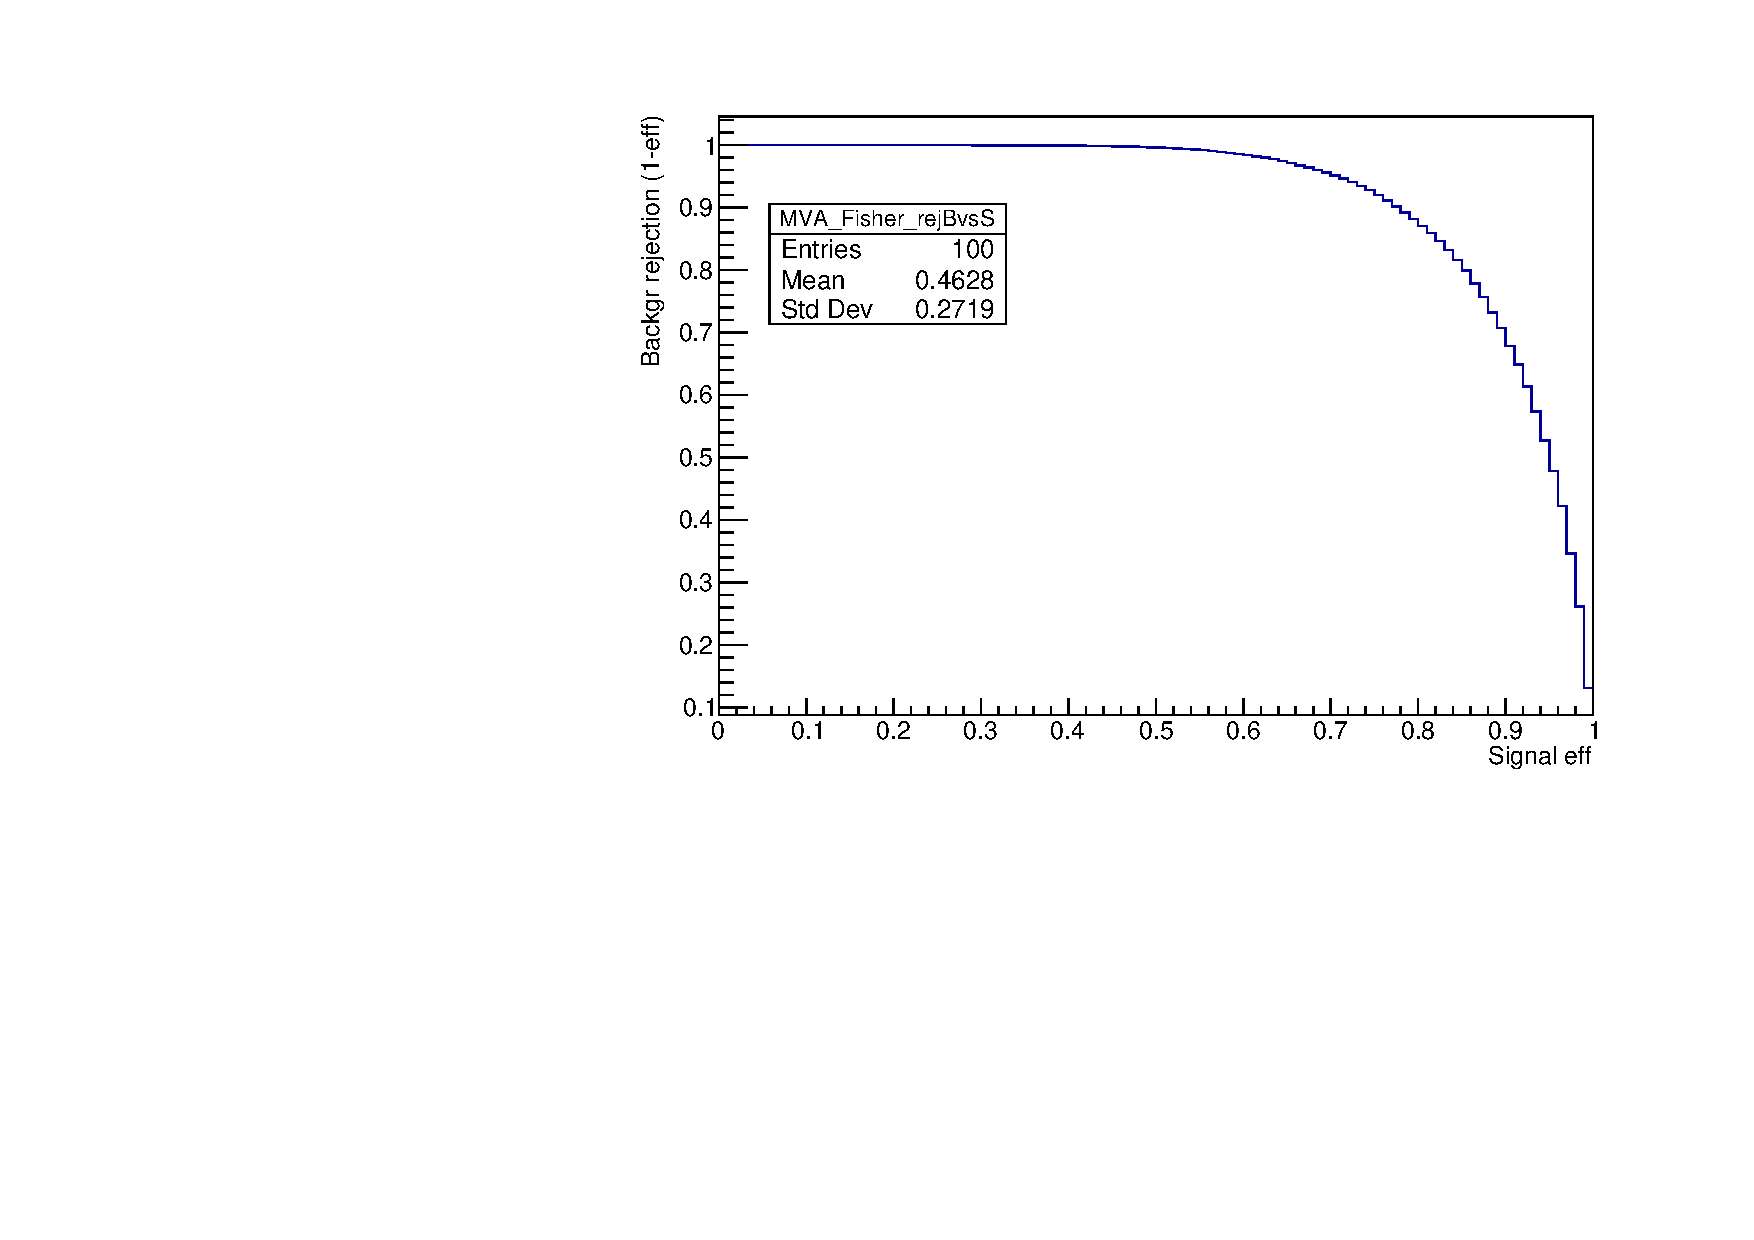
\includegraphics[width=8cm]{fisher_auc.pdf}
	\caption{ROC curve of Fisher discriminant.}
	\label{fisher_auc}
\end{figure}

\begin{table}[ht]
	\centering
	\caption{Testing results from different TMVA methods.}
	\label{table:tmvaMethod}
	\begin{tabular*}{100mm}{c@{\extracolsep{\fill}}ccc}
		\toprule
		Method & AUC &CPU time (sec) \\
		\hline 
		\multicolumn{3}{|l|}{Energy [4,15] MeV}
		\midrule
		Fisher &  & 0.2\\
		Likelihood &   &0.2\\
		BDT & & \\
		BDT-B& & \\\
		MLP & & 767 \\
		\bottomrule
	\end{tabular*}
\end{table}

A quantity called Area Under the Curve (AUC) is often used to summarize the quality of a ROC curve\cite{murphy2012machine}. 


ROC curve 0.915


%energy cuts, ts combining with NHit cuts

%6 variables used as inputs


The distributions of $\cos\theta_{sun}$ were used to show the performance of the solar $\nu_e$ event selection and background event discrimination. 

\begin{figure}[!htb]
	\centering
	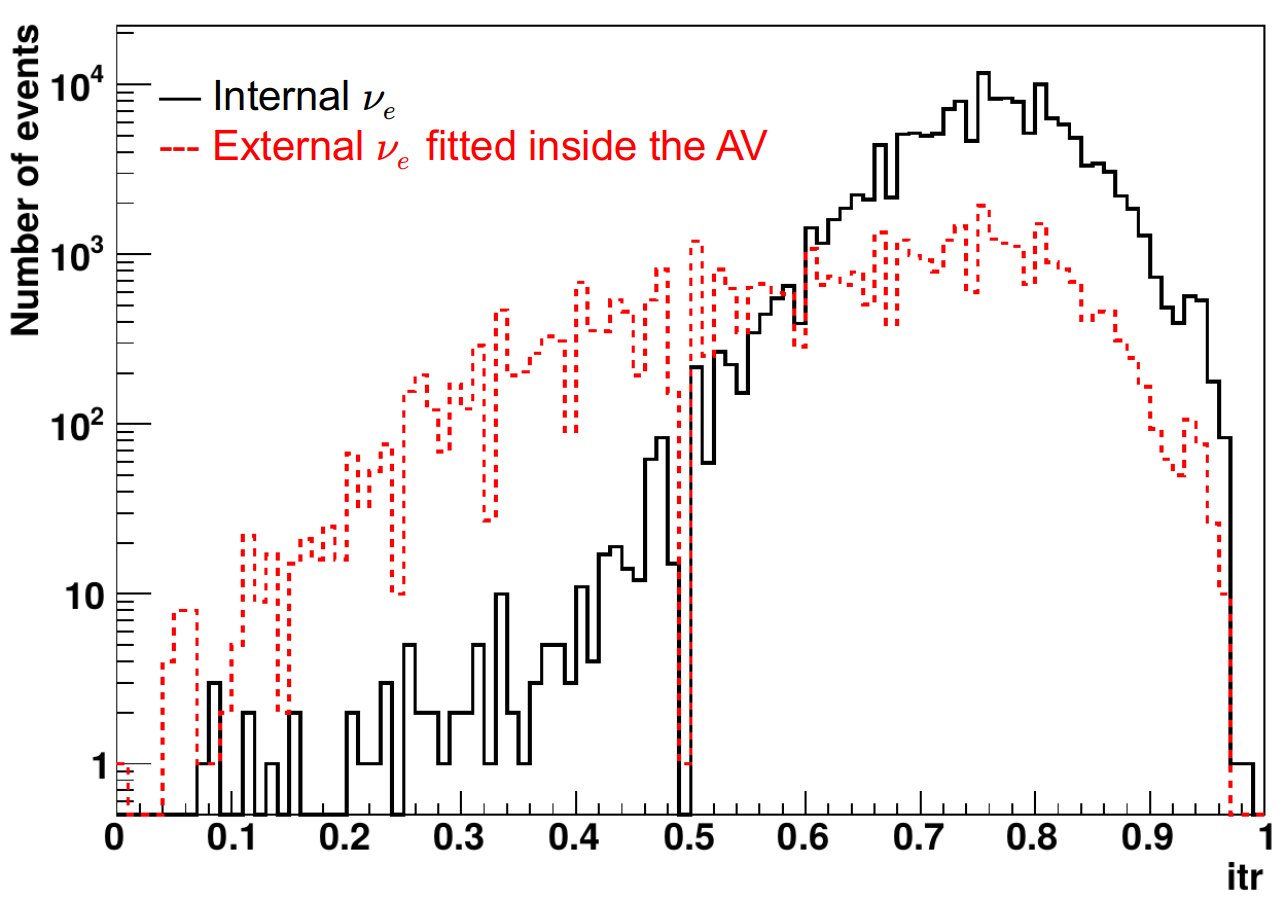
\includegraphics[width=8cm]{ITR_MPW_solarNuVsExSolar.png}
	\caption{Comparison between solar $\nu_e$ and external solar $\nu_e$; MPW results.}
	\label{itrCmp}
\end{figure}

Other packages developed for high energy particle physics, such as StatPatternRecognition (SPR)\cite{sprWebsite}, can be considered as an alternative tool or as a reference for results comparisons. 

\subsection{Likelihood Fits for Solar Neutrino Candidate Events}
The optimized cuts obtained from the TMVA analysis from the previous section were applied on the dataset. 

After the event selections, a distribution of $\cos\theta_{sun}$ extracted from the solar $\nu_e$ candidate events was obtained. 

\subsubsection{Maximum Likelihood Fit}
A maximum likelihood method was applied on the distribution to extract the number of the solar $\nu_e$ events ($N_{sig}$) as well as the number of the background events ($N_{bkg}$).

The values of $\cos\theta_{sun}$ from the selected events were filled into a histogram divided into bins.
For each bin, the observed event number ($n_{obs}$) was considered as a sum of solar $\nu_e$ and background events. The $n_{obs}$ in each bin was assumed to follow a Poisson distribution: $Poisson(n_{obs}, N_{bkg}\cdot P_{bkg}+N_{sig}\cdot P_{ES}(E))$, where $P_{bkg}$ and $P_{ES}(E)$ are the assumed distribution of backgrounds and solar $\nu_e$ events respectively.

For the background events, a uniform distribution of $\cos\theta_{sun}$ was assumed. On the other hand, the $\cos\theta_{sun}$ distribution of solar $\nu_e$ was extracted from the realistic simulations after applying the optimized cuts, as shown in Fig.~\ref{solarPDF}. 

\begin{figure}[!htb]
	\centering
	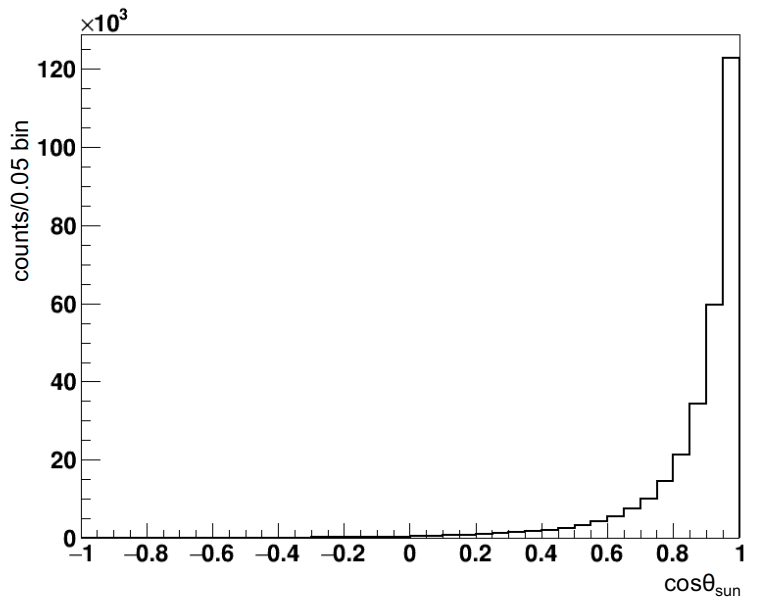
\includegraphics[width=8cm]{solarPDF.png}
	\caption{The $\cos\theta_{sun}$ distribution of solar $\nu_e$ extracted from the simulations, which was used as a pdf function.}
	\label{solarPDF}
\end{figure}

Adding up each bin $i$ and taking $N_{bkg}$ and $N_{sig}$ as fit parameters, the maximum likelihood function was built as:
\begin{equation}\label{eq:solar_poissonFit}
-\ln\mathcal L(N_{signal},N_{bkg}|n_{obs})
=-\sum_i\ln(Poisson(n^i_{obs}, N_{bkg}P^i_{bkg}+N_{sig}P^i_{ES}(E^i))),
\end{equation}

By fitting the \ref{eq:solar_poissonFit} to the data, $N_{bkg}$ and $N_{sig}$ were obtained.
Fig.~\ref{solarFits1} shows the fit results. The fitted number of solar $\nu_e$ events is $N_{sig} = 67.1\pm9.2$, which is equivalent to a rate of $1.04\pm 0.14~event/(day\cdot kiloton)$; while the fitted number of background events is $N_{sig} = 3.4\pm0.91$, which is equivalent to a rate of $0.05\pm 0.01 event/(day\cdot kiloton)$.

\begin{figure}[!htb]
	\centering
	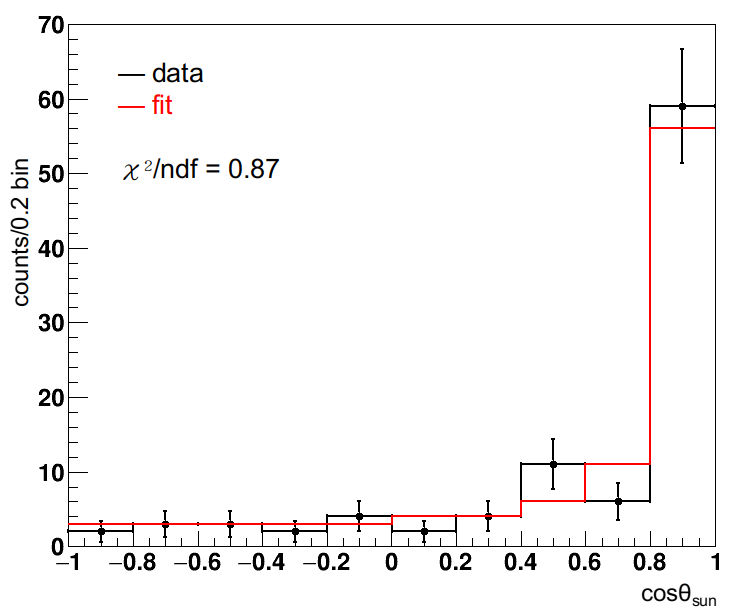
\includegraphics[width=8cm]{solarFits1.png}
	\caption{Fitted results for the $N_{bkg}$ and $N_{sig}$ via the maximum likelihood method.}
	\label{solarFits1}
\end{figure}

2D fits



\subsubsection{Systematics Evaluation}
The systematics of position, direction and energy reconstruction were obtained from the Chapter 5.

